%\section{Casistiche di utilizzo della base di dati}

%-	Quando un utente va via dovrà quindi pagare il conto, che è la somma di tutti i servizi di cui ha usufruito
%-	Avere facilmente in vista tutte le persone all’interno del marina
%-	Conoscere rapidamente quanti posti disponibili relativamente a certe dimensioni ci sono
%-	Ottenere i dati necessari a compilare i documenti doganali e relativi al soggiorno in uno stato estero per gli utenti con nazionalità differente dal marina


\section{Query}

\subsection{Consumi del marina nel mese indicato}
\begin{lstlisting}
--Calcola consumi del marina nel mese indicato

select allacciamento,
       sum(quantita) as quantita_consumata,
       a.unitamisura, a.prezzounitario,
       sum(quantita) * a.prezzounitario as totale_bollette
from consumo
join allacciamento a on consumo.allacciamento = a.nome
where inizio between '05-01-2020' and '05-31-2025'
group by allacciamento, unitamisura, prezzounitario;

\end{lstlisting}

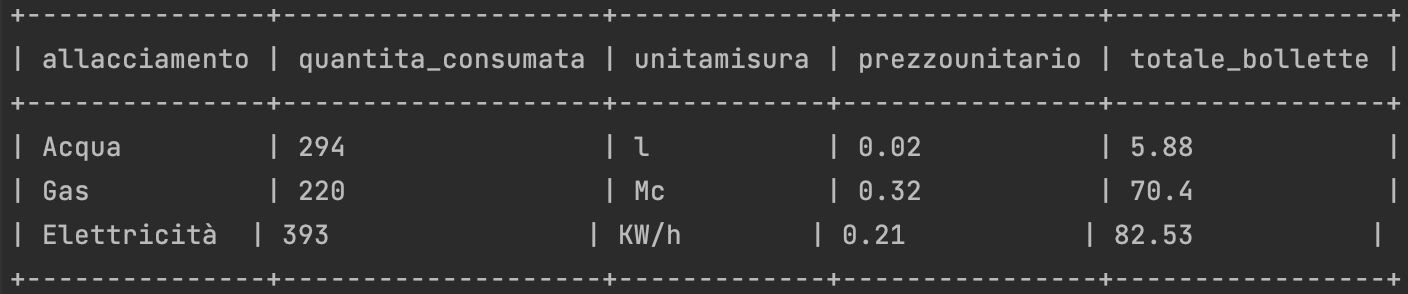
\includegraphics[width=\linewidth]{img/result_consumi.png}

\subsection{Clienti con più di 2 di prenotazioni che iniziano nel quinquiennio 2020->2025}

\begin{lstlisting}
--Ritorna i clienti con più di 2 di prenotazioni che iniziano nel quinquiennio 2020->2025
--Questa query è utile in ottica di creazione di uno sconto per chi fa molte prenotazioni

select count(cliente) as conteggio, p.nome, p.cognome, c.persona
from prenotazione
join cliente c on prenotazione.cliente = c.id
join persona p on c.persona = p.cf
where prevarrivo between '01-01-2020' and '12-31-2025'
group by c.persona,p.nome, p.cognome
having count(cliente) >= 2
order by conteggio desc;
\end{lstlisting}

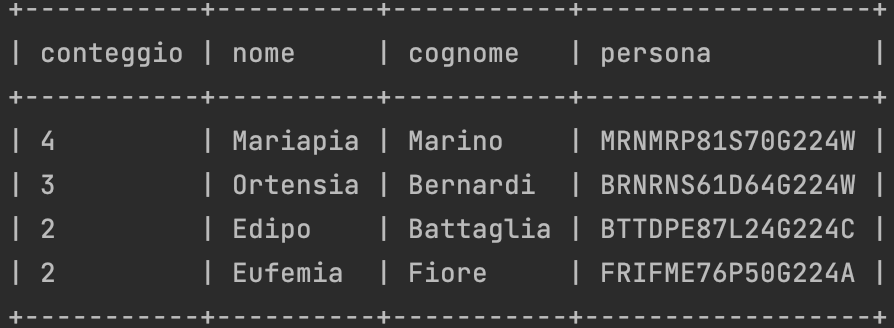
\includegraphics[width=\linewidth]{img/result_2prenotazioni.png}

\subsection{Conteggio soste di ogni imbarcazione}

\begin{lstlisting}
--Conteggia le soste delle imbarcazioni

select count(imbarcazione) as qt_soste, imbarcazione.nome, mmsi,p.nome as nome_proprietario,p.cognome as cognome_proprietario
from sosta
join imbarcazione on sosta.imbarcazione = imbarcazione.id
join cliente c on imbarcazione.cliente = c.persona
join persona p on c.persona = p.cf
group by sosta.imbarcazione, imbarcazione.nome, mmsi,p.nome,p.cognome
order by qt_soste desc;
\end{lstlisting}

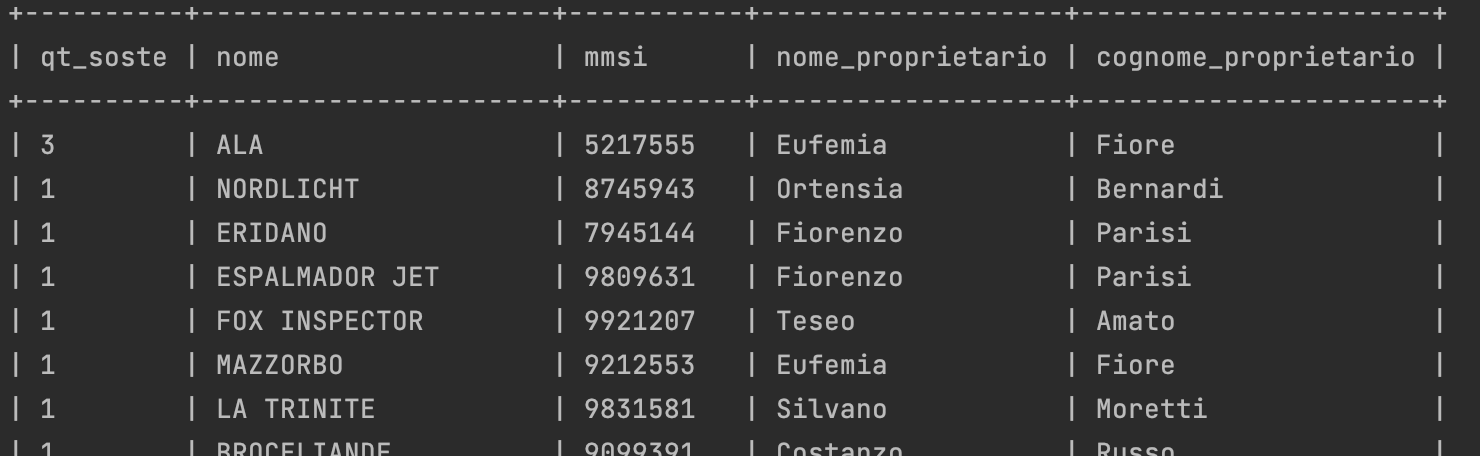
\includegraphics[width=\linewidth]{img/result_sosteimb.png}

Il risultato contiene tante righe quante le imbarcazioni, è stato quindi troncato per limitare il consumo di spazio.

\subsection{Controllo dei posti disponibili per una certa imbarcazione}
\begin{lstlisting}
--controllo dei posti disponibili per una certa imbarcazione

select distinct molo.id as id_molo,molo.prezzogiorno,
    molo.profonditaminima,molo.larghezza,molo.lunghezza, molo.occupato
from molo,imbarcazione
where occupato=false
and molo.larghezza > imbarcazione.larghezza
and molo.profonditaminima > imbarcazione.pescaggio
and molo.lunghezza > imbarcazione.loa
and imbarcazione.mmsi = '8836340'
order by prezzogiorno
limit 5;
\end{lstlisting}

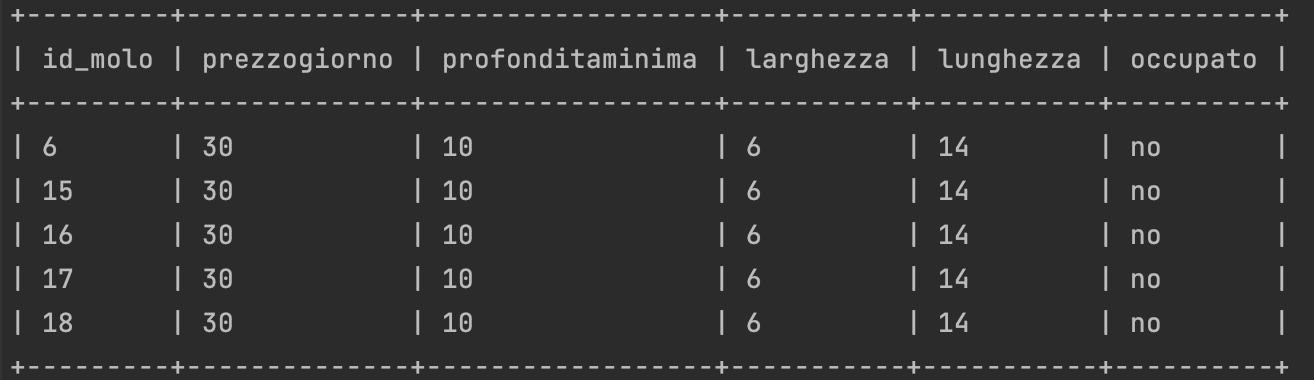
\includegraphics[width=\linewidth]{img/result_molidisponibili.png}

\subsection{Stampa fattura di un cliente}

\begin{lstlisting}
 -- stampa la fattura di un cliente

with intestazione_fattura as(
    select fattura.*, p.nome, p.cognome from fattura
    join cliente c on c.persona = fattura.cliente
    join persona p on c.persona = p.cf
    where cliente = 'GLLGNN81A54G224W'),

spese as(
    select sosta.fattura,
            i.cliente,
            'sosta' as tipo,
            ROUND((tstzrange_subdiff(sosta.partenza,sosta.arrivo)
            /86400.0 * m.prezzogiorno)::numeric,2)  as prezzo
    from sosta
    join imbarcazione i on i.id = sosta.imbarcazione
    join molo m on sosta.molo = m.id
    where partenza != 'infinity'

    union all
    select consumo.fattura,
            consumo.cliente,
            'consumo' as tipo,
            ROUND((consumo.quantita * a2.prezzounitario)::numeric,2) as prezzo
    from consumo
    join fornitura f on consumo.allacciamento = f.allacciamento
    join allacciamento a2 on consumo.allacciamento = a2.nome
)

select distinct id, scadenza, pagato, nome, cognome,
    intestazione_fattura.cliente, tipo, prezzo
from spese, intestazione_fattura
where spese.fattura = intestazione_fattura.id;
\end{lstlisting}

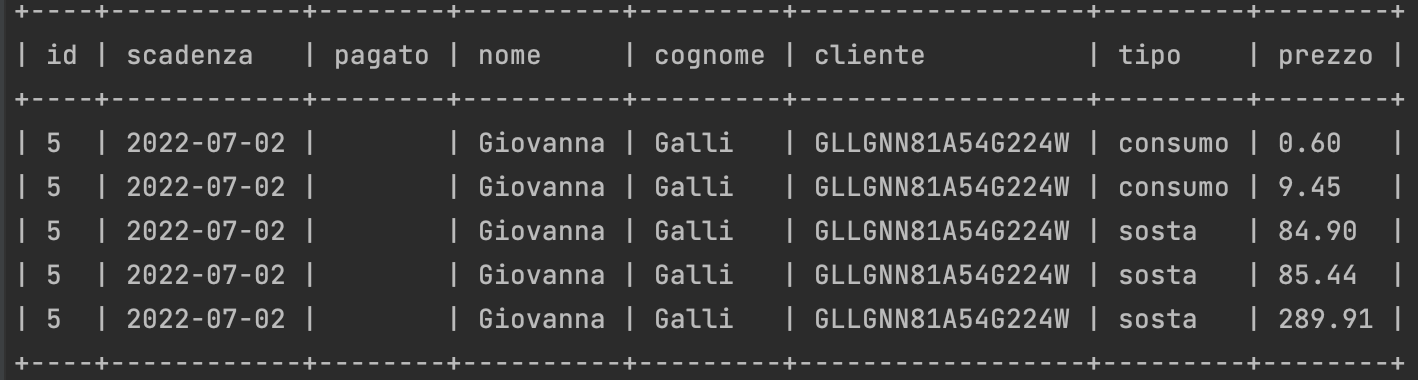
\includegraphics[width = \linewidth]{img/result_fattura.png}

\section{Indicizzazione}

Essendo modificata pochissime volte\footnote{Ovvero solo in caso di ristrutturazioni del marina} e letta spesso in moltissime operazioni, l'entità \textbf{Molo} è importante che venga indicizzata tramite B-Tree, in questo modo, entrando per mezzo dell'id sarà decisamente più efficiente leggerne attributi come ad esempio le dimensioni o lo stato di occupazione.

L'indice appena descritto sarebbe poi comunque utile anche in caso di utilizzo su larga scala con migliaia di moli, oppure nel caso si volesse adattare la base dati all'utilizzo con una serie marina contenenti molti moli. I risultati di efficienza aumentata sarebbero quindi ancora più evidenti e utili.

Sono stati poi, come precedentemente descritto al punto \ref{vincoli_gestiti} , utilizzati dei search tree per utilizzare al meglio i costraint relativi alle date ed orari di \textbf{prenotazioni} e \textbf{soste}.
